\documentclass[11pt]{article}
\usepackage[final]{acl}
\usepackage{fontspec}
\usepackage{latexsym}
\usepackage{graphicx}
\usepackage{tabularx}
\usepackage{booktabs}   % for \toprule, \midrule, \bottomrule
\usepackage{multirow}   % for \multirow
\usepackage{algorithm}
\usepackage{amssymb}
\usepackage{zi4} 
\usepackage{algpseudocode}
\usepackage{amsmath}
\usepackage{enumitem}
\usepackage{float}
\usepackage{varwidth}
\usepackage{svg}
\usepackage{hyperref}
\usepackage{microtype}
\usepackage{subcaption}
\usepackage{polyglossia}
\setdefaultlanguage{english}
\setotherlanguages{tamil}
\setmainfont{TeX Gyre Termes}
%\setmonofont{Inconsolata}
\newfontfamily{\tam}[Script=Tamil, Scale=0.60]{nirmala.ttf}
\newfontfamily{\prompt}[Script=Latin, Scale=0.6]{RobotoMono-Light.ttf}
\usepackage{array, booktabs, makecell, multirow, tabularx, siunitx, etoolbox, expl3}
\usepackage{geometry}
\geometry{margin=1in}
\usepackage{adjustbox}
\usepackage{expl3}
\usepackage{pgfplots}
\usepackage{tikz}
\renewcommand\theadfont{\bfseries\small}
\renewcommand\arraystretch{0.83}
\setlength{\tabcolsep}{20pt}
\sisetup{
  round-mode=places,
  round-precision=3,
  detect-weight=true,
  detect-family=true,
  table-align-text-post=false
}
\newcolumntype{Z}{>{\centering\arraybackslash}X}
\newcolumntype{s}{>{\centering\arraybackslash\hsize=1.2\hsize\collectcell\siunitxnumber}X<{\endcollectcell}}

\title{\emph{VIDAI}: VIDukathAI Interpretation Through Analysis of In-context Reasoning in Tamil using LLMs}

\author{
R S Mughil Srinivasan$^{1}$ \\
106122104@nitt.edu 
\And
Kesavan T$^{1}$ \\
106122068@nitt.edu
\And
Abhijith Balan$^{1}$ \\
406123001@nitt.edu
\AND
Abhinav P M$^{2}$ \\
abhinav.pm@research.iiit.ac.in
\And
Parameswari Krishnamurthy$^{2}$ \\
param.krishna@iiit.ac.in
\\[0.5em]
\textsuperscript{1}National Institute of Technology, Tiruchirappalli \\
\textsuperscript{2}International Institute of Information Technology, Hyderabad \\
\And
Oswald C$^{1}$ \\
oswald@nitt.edu
}
\begin{document}
\maketitle


\begin{abstract}
This work investigates VIDAI, a study on Tamil vidukathai, where \textit{vidai} means `answer' and \textit{vidukathai} means `riddle' in the Tamil language, focusing on the challenges Large Language Models (LLMs) face in solving them. Tamil, a morphologically rich and culturally embedded classical Dravidian language of India, with over 2000 years of history, is spoken officially in three countries and across global diaspora communities. Although models such as LLaMA, Phi, Gemma, and Qwen excel in general NLP tasks, they struggle with Tamil riddles due to their reliance on next-token prediction and limited reasoning ability. Tamil riddles frequently use metaphors, puns, cultural references, and abstract logic, posing difficulties for models trained primarily on generic corpora. We curated a dataset of 2,283 riddles\footnote{\url{https://anonymous.4open.science/r/TamilRiddlesDataset-48C3}} and evaluated the models under various prompting strategies. The highest performance achieved was a BERTScore of 0.846 with a random 1-shot no-CoT prompt. VIDAI's findings highlight riddles as a promising benchmark for testing reasoning in LLMs.
\end{abstract}
\paragraph{Keywords:}  CoT, In-Context Learning, LLM, Question Answering, Riddle, Tamil 

\section{Introduction}
Large Language Models (LLMs) such as GPT, LLaMA, Phi, and Gemma have advanced natural language processing, excelling in summarization, translation, question answering, and text generation \cite{sanchez-bayona-agerri-2025-metaphor, tong-etal-2024-metaphor, giadikiaroglou-etal-2024-puzzle, jiang-etal-2023-brainteaser}. These strengths stem from large-scale pretraining and fine-tuning on diverse datasets. However, LLMs struggle with tasks that require symbolic abstraction, associative reasoning, and cultural grounding, such as solving a riddle ~\cite{liu2024multilingualllmsculturallydiversereasoners}.

LLMs are trained on next token prediction objectives ~\cite{lin2025reasoningbiastokenprediction}, favoring high-frequency, contextually probable outputs. Although effective for factual tasks, this biases models against riddles, which rely on ambiguity, metaphor, and wordplay. Solving riddles requires inference, analogy, and creative abilities that were not explicitly learned during training.

These challenges are amplified in morphologically rich and culturally grounded languages such as Tamil. With more than 2000 years of literary history, Tamil has agglutinative morphology, rich inflections, eight grammatical cases ~\cite{lehmann1993grammar}, and distinctive phonology documented in the \textit{Tolkāppiyam} \cite{tolkappiyam}. Its oral traditions feature riddles (\textit{Vidukathai} in Tamil language) using metaphors, puns, idioms, and poetic conventions such as \textit{venpa}, \textit{ullurai}, and \textit{iraicchi} ~\cite{schiffman1999spoken,purapporulvenbamaalai}. These cultural markers are rarely present in large corpora in English, causing models to default to generic or plausible answers.

VIDAI introduces the first dedicated Tamil riddles dataset, providing a benchmark to evaluate LLM performance by inferring and understanding Tamil riddles, and assesses open-source models using structured prompting, semantic example selection, and multi-metric evaluation. VIDAI's study highlights reasoning gaps and conditions that improve model performance, offering insight into handling metaphor-rich, culturally specific tasks.

The paper is organized as follows: \S 1 introduces the motivation, contributions, and problem statement. Related riddle-solving and multilingual LLM reasoning work are reviewed in \S 2. \S 3 explains the creation of the Tamil Dataset. The details of the design of VIDAI and the prompting strategies are explained in \S 4. \S 5 discusses the evaluation,  metrics, and observations of the experiments. \S 6 presents the key takeaways. The conclusion and directions for future work are presented in \S 7.

\subsection{Contributions}
\begin{itemize}
    \item \textbf{Dataset Creation:} Compiled a cleaned dataset of 2,250+ Tamil riddles from books and public sources, categorized into Objects, Nature, Actions, People, and Abstract Concepts.
    \item \textbf{Few-Shot Prompting and CoT:} Designed random and semantically similar few-shot settings (1, 2, 3, 5 shots) and generated CoT explanations using ChatGPT for selected examples and manually curated to ensure alignment with human interpretations in solving a riddle.
    \item \textbf{Multi-Metric Evaluation:} Used Exact Match, Levenshtein Distance, and BERTScore to assess both literal and semantic correctness.  
    \item \textbf{Local LLM Execution:} Ran experiments on Phi-4, Gemma2: 9b, Gemma3.1: 12b, LLaMA3: 8b and Qwen2.5: 7b via Ollama\footnote{\url{https://ollama.com/}}.  
    \item \textbf{Riddle Reasoning in Tamil:} Focused on metaphor-rich riddles in a low-resource language to test cultural and linguistic reasoning.  
\end{itemize}

\subsection{Problem Description}
LLMs excel at next-token prediction, favoring common, contextually likely continuations, which suits tasks like summarization or dialogue. However, the riddles are based on misdirection, wordplay, and layered meanings, demanding abstraction and creative reasoning. Tamil riddles add challenges with cultural references, phonetic puns, and idioms, rare in mainstream corpora, reducing model effectiveness, and highlighting a gap in multi-step, metaphorical reasoning.

The problem statement is defined as follows: Let \(\mathcal{R} = \{(r_1, a_1), (r_2, a_2), \dots, (r_n, a_n)\}\) be a collection of Tamil riddles, where each \(r_i\) represents a riddle, \(a_i\) - its corresponding answer, and \(n = |\mathcal{R}|\), for \(1 \leq i \leq n\). The task is to curate \(\mathcal{R}\), then evaluate a series of Large Language Models to answer the riddles by predicting an answer \(b_i\) and computing the similarity of (\(b_i\), \(a_i\)) with the help of various metrics.

\section{Related Work} 
Recent studies have begun to treat riddle solving as a test of LLM reasoning. \cite{panagiotopoulos-etal-2025-riscore} proposed a context-reconstructed augmentation method that improves performance by providing structurally similar riddles as few-shot prompts. However, their work focuses on multiple-choice formats rather than VIDAI's method of QA style. \cite{giadikiaroglou-etal-2024-puzzle} survey puzzles, classifying them into rule-based and rule-less forms, and note that the riddles remain challenging for LLMs. Although they call for better datasets and hybrid methods, their analysis is largely language-agnostic and not tailored to low-resource languages.
\cite{lin-etal-2021-riddlesense} and \cite{jiang-etal-2023-brainteaser} address commonsense and linguistic creativity in English riddles and lateral puzzles. However, their methods are language-specific and do not address metaphor in non-English contexts. Similarly, \cite{tan-etal-2016-solving} tackles the Chinese character riddles using language-specific fine-tuning, limiting cross-lingual applicability. Few-shot learning studies \cite{brown2020languagemodelsfewshotlearners, agarwal2025manyshotincontextlearning} informed VIDAI's shot size design, while \cite{wei2022cotpromptingelicitsreasoninginllms} inspired VIDAI's CoT approach. However, these works primarily test English tasks. \cite{zhang2022birdqabilingualdatasetquestion} and \cite{xu2023ccriddlequestionansweringdataset} confirm riddles as multilingual challenges but focus on multiple-choice formats, unlike VIDAI's QA format.
The work of \cite{liu-etal-2022-makes} validates the benefit of semantically similar examples, aligning with VIDAI's sampling strategy. Reasoning-oriented prompting research \cite{kojima2022largelanguagemodelsarezeroshotreasoners, fu2023complexitybasedpromptingmultistepreasoning} offers useful insights, but is based on mathematical and logic puzzles. Theoretical studies \cite{jerome2024inductivereasoninginhumansandllms, wei2022emergentabilitieslargelanguage} explore general reasoning but neglect the resolution of culturally rich metaphors. In general, no major study goals are open in any Indian language, such as Tamil, which requires deep cultural and symbolic reasoning.

\section{Dataset Creation}
\subsection{Dataset Sources}
We collected the Tamil riddle dataset from various public sources, including books and online repositories. The sources are from classical Tamil riddle books such as \cite{1000tamilriddlesbook} and \cite{500tamilriddlesbook}. We incorporate riddles from educational websites such as ~\cite{vidukathaitamil}, \cite{tamilvidukathaigal2020}, \cite{tamilvidukathaigal2024}, and quiz portals such as \cite{tamilvidukathaigalquiz} and \cite{tamilmolzigalvidukathaigal}. The VIDAI's final dataset consisted of 2,283 unique Tamil riddles, each paired with a single ground-truth answer. This represents the largest available collection of Tamil riddles from which we could extract the best from online sources.

\subsection{Riddle Structure}
Riddles ranged from one to five poetic lines in colloquial Tamil, with answers as single words or short phrases. While some mapped to concrete concepts, others required abstract or symbolic interpretation.

\subsection{Categorization of Riddles}
We classified VIDAI's dataset based on the Tamil riddle answers into five broad semantic categories.
\begin{itemize}
\item \textbf{Natural Elements and Weather}: Answers related to natural phenomena and cycles, often expressed through environmental metaphors. Examples: {\tam சூரியன்} - (Sūriyaṉ, Sun), {\tam காற்று} - (Kātṟu, Wind).
\item \textbf{Human Body and Senses}: Refers to body parts or sensory actions, typically using anatomical or functional metaphors. Examples: {\tam மூச்சு} - (Mūccu, Breath), {\tam நாக்கு} - (Nākku, Tongue).
\item \textbf{Objects and Tools}: Man-made items are described through their form, function, or purpose. Examples: {\tam நாற்காலி} - (Nāṟkāli, Chair), {\tam கடிகாரம்} - (Kaṭikāram, Clock).
\item \textbf{Food and Plants}: Edible items or plants, often described using taste, texture, or appearance. Examples: {\tam வெங்காயம்} - (Veṅkāyam, Onion), {\tam கரும்பு} - (Karumpu, Sugarcane).
\item \textbf{Animals and Insects}: Creatures referenced through behavior, sounds, or cultural associations. Examples: {\tam சிலந்தி} - (Silanti, Spider), {\tam நாய்} - (Nāy, Dog).
\end{itemize}

\begin{figure*}[h]
  \centering
  \makebox[\textwidth][c]{%
    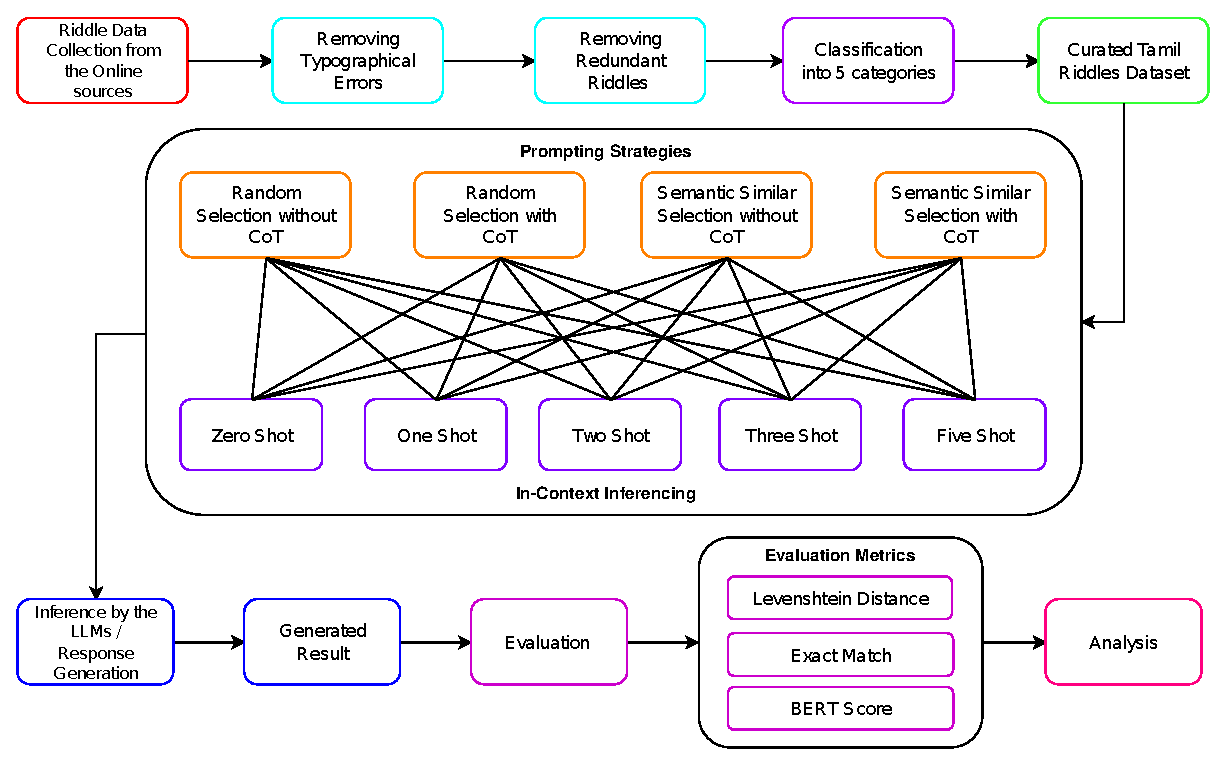
\includegraphics[width=1\textwidth]{testv3.eps}
  }
  \caption{Architecture diagram of VIDAI: VIDukathAI Interpretation Through Analysis of In-context Reasoning in Tamil using LLMs}
  \label{fig:ArchitectureDiagram}
\end{figure*}

\section{Design}
Figure~\ref{fig:ArchitectureDiagram} shows the architecture of VIDAI, using five open-source LLMs: LLaMA 3.1 (8B), Phi-4, Gemma 2 (9B), Gemma 3.1 (12B), and Qwen 2.5 (7B) with zero, one, and few-shot prompting. In few-shot settings, the models received 2, 3, and 5 riddle-answer examples.  

We employ two sampling strategies: Random Sampling and Semantic Similarity Sampling. In Random Sampling, examples were selected arbitrarily from the training set, with each example likely originating from a different class. In contrast, Semantic Similarity Sampling involved first selecting one of the five predefined categories, established through manual classification of the dataset based on the answers, as described in Section \textit{Categorization of Riddles}, and then randomly drawing all examples from that category. For instance, in a three-shot prompt, Random Sampling would yield three examples from potentially different categories, whereas Semantic Similarity Sampling would select a single category at random and then draw three examples exclusively from it.

\subsection{Chain-of-Thought}
Initially, the examples included only riddle-answer pairs. In a second phase, we extended the prompts using \textbf{Chain-of-Thought (CoT)} reasoning, adding explanatory reasoning to each example. CoT explanations were presented in a consistent deductive format in all examples. Each riddle is first restated and explained in English, followed by the revelation of the answer. The explanation then proceeds by mapping each segment of the riddle to its underlying meaning, interpreting phrases in relation to the proposed answer, and the justification explicitly shows how the answer satisfies each part of the riddle. This ensures that the meanings embedded in figurative, metaphorical, or cultural contexts are extracted and clarified.  The length of the explanations naturally varies according to the complexity of the riddle.

\subsection{Direct Prompting}
In this setup, the model was given only the riddle, without any additional guidance, and tasked with producing an answer. This zero-shot approach relies entirely on the internal knowledge and reasoning of the model to interpret and solve the riddle.

An example prompt given without CoT explanation : 

\texttt{Provide only the final answer in Tamil without any translations or explanations in English for the given Tamil riddle below.}

\texttt{Question : }{\tam பறக்கும் ஆனால் பறந்து போகாது, அது என்ன?} 

\texttt{Answer:}

\subsection{Few-Shot Prompting}
We adopt a few-shot strategy with Chain-of-Thought (CoT) reasoning, where each example includes the riddle, its answer, and step-by-step reasoning to interpret metaphors, recognize symbols, and eliminate unlikely options. These CoT explanations, generated using ChatGPT-4o with the riddle and its known answer, were then manually curated to ensure coherence, contextual relevance, logical foundation and alignment with human interpretations.

An example of a 1-shot prompt given with CoT explanations is: 

\texttt{Question:} {\tam வீட்டுக்குள்ளே இருப்பாள், விந்தையாகப் பேசுவாள், வந்தவரை வா என்பாள், வாசல் தாண்டிப் போகமாட்டாள். அவள் யார்?}

\texttt{Answer: }{\tam நாக்கு}

\texttt{Explanation: The riddle describes something that stays inside the house, speaks mysteriously, invites people, and never crosses the threshold. The answer is {\tam நாக்கு} (tongue). }{\tam வீட்டுக்குள்ளே இருப்பாள்}\texttt{ refers to the tongue that remains inside the mouth (the house). }{\tam விந்தையாகப் பேசுவாள்}\texttt{ highlights its role in speaking, }{\tam வந்தவரை வா என்பாள்}\texttt{ shows how it welcomes speech, and }{\tam வாசல் தாண்டிப் போகமாட்டாள்}\texttt{ means it never leaves the mouth.}

\texttt{Provide only the final answer in Tamil without any translations or explanations in English for the given Tamil riddle below.}

\texttt{Question: }{\tam பாதுகாப்பான பெட்டிக்குள்ளே பலரும்‌ விரும்பும்‌ கடிகாரம், அது என்ன?} 

\texttt{Answer:}

Enriched examples are especially useful for solving riddles, where metaphorical and cultural understanding is the key. Comparing these two prompting approaches helps evaluate how in-context learning and example-based reasoning affect LLM performance on complex, ambiguous queries. All experiments were run locally using models downloaded via Ollama, depending on available resources.

\section{Evaluation, Results and Observations}
To assess model performance in solving Tamil riddles, we employed four key evaluation metrics, each capturing different aspects of answer quality:

\begin{itemize}
\item \textbf{Exact Match:}  
Checks if the model answer exactly matches the ground truth. It is simple but rigid, often penalizing correct synonyms or alternate Tamil wordings.
It is defined as:

$\text{Exact Match (EM)} = \frac{\sum_{i=1}^{N} \mathbb{1}[\hat{y}_i = y_i]}{N}$

\item \textbf{Levenshtein Distance:}  
Measures similarity via minimal character edits, normalized as [0, 1]. It detects typos and near matches, but misses semantically correct words with different spellings.  
It is defined as:

$\text{Levenshtein Similarity} = 1 - \frac{d_{\text{lev}}(\hat{y}, y)}{\max(|\hat{y}|, |y|)}$

\item \textbf{BERTScore:}  
Uses transformer embeddings to compare tokens, capturing semantic meaning and paraphrases, effective for Tamil riddles with subtle contextual nuances.
It is defined as:

$\text{BERTScore}_{F1} = \frac{1}{N} \sum_{i=1}^{N} F1(\hat{y}_i, y_i)$
\end{itemize}

Tamil riddles, rich in metaphor and cultural nuance, require evaluation beyond strict string matching. We use BERTScore with surface metrics to capture semantic equivalence across varying wordings, analyzing the effects of context, model size, and explanation style across multiple prompting setups.

\subsection{Algorithm Trace Example}
This section presents a sample execution of Algorithm~\ref{alg:algorithm} for one configuration. The model is Phi-4, using the \textit{Semantic similarity} prompting strategy with 3 shots. The test riddle is {\tam மேலே மேலே போகும், கீழே கீழே போகாது. என்ன?} (Mēlē mēlē pōkum, kīḻē kīḻē pōgātu. Eṉṉa?) – It keeps going upward, but never goes downward. The ground truth answer is {\tam வயது} (Vayatu) – Age. The evaluation begins with \texttt{GetFewShotExamples(model, riddle, shot=3, strategy="semantic")}, which selects three semantically related examples, focusing on abstract concepts from \textit{Human Body \& Senses} category. Then, \texttt{LoadTestSet()} loads the riddle and its ground truth answer.  Next, \texttt{ConstructPrompt(few\_shot\_examples, test\_riddle)} builds the prompt by combining the examples with the target riddle in QA format. Passing this on to \texttt{GenerateAnswer(model, prompt)} yields {\tam புகை} (Pogaei) – Smoke. Although incorrect, this highlights the model’s reliance on surface-level cues rather than abstract temporal reasoning. Finally, \texttt{Evaluate()} computes metrics such as \textit{BERTScore}, reflecting partial semantic proximity in the metaphorical interpretation between smoke and age.
\begin{algorithm}
\footnotesize
\caption{Evaluate Models on Riddle QA with Few-Shot Prompts}
\label{alg:algorithm}
\begin{algorithmic}[1]
\State \textbf{Input:} \textit{TestSet}, \textit{FewShotData}, \textit{ShotCounts}, \textit{Models}, \textit{PromptModes}
\vspace{0.5em}
\ForAll{Model $\in$ Models}
    \State Load model via local or remote interface
    \vspace{0.1em}
    \ForAll{PromptMode $\in$ PromptModes}
        \ForAll{ShotCount $\in$ ShotCounts}
            \vspace{0.1em}
            \If{ShotCount $>$ 0}
                \State \parbox[t]{\linewidth}{%
                    Examples $\gets$ \texttt{GetFewShotExamples}(\\
                    FewShotData, PromptMode, \\
                    ShotCount)%
                }
            \Else
                \State Examples $\gets \emptyset$
            \EndIf
            \vspace{0.1em}
            \State \parbox[t]{\linewidth}{%
                $(\text{Questions}, \text{Answers}) \gets$ \texttt{LoadTestSet}\\
                (TestSet)%
            }
            \State Predictions $\gets$ [ ]
            \vspace{0.1em}
            \ForAll{Question $\in$ Questions}
                \State \parbox[t]{\linewidth}{%
                    Prompt $\gets$ \texttt{ConstructPrompt}(\\
                    Examples, Question, PromptMode)%
                }
                \State \parbox[t]{\linewidth}{%
                    Response $\gets$ \texttt{GenerateAnswer}(\\
                    Model, Prompt)%
                }
                \State Append Response to Predictions
            \EndFor
            \vspace{0.1em}
            \State \parbox[t]{\linewidth}{%
                Metrics $\gets$ \texttt{Evaluate}(Predictions,\\
                Answers)%
            }
            \vspace{0.5em}
            \State \textbf{Evaluation Metrics:} \textit{Exact Match}, \textit{Cosine Similarity}, \textit{BERTScore}, \textit{Levenshtein Similarity}
        \EndFor
    \EndFor
\EndFor
\end{algorithmic}
\end{algorithm}

\subsection{Results and Discussions}
We ran the five open-source LLMs on 14th Gen Intel Core i7 CPU, NVIDIA T1000 8 GB GPU with 16 GB Main Memory and 512 GB Hard Disk on Linux platform using Python code. The models LLaMA 3.1 (8B), Phi-4, Gemma 2 (9B), Gemma 3.1 (12B), and Qwen 2.5 (7B) were evaluated across four setups: semantically similar or random riddles, with or without CoT explanations, under zero, one, and few-shot (2, 3, 5) conditions. Performance was measured using exact match, Levenshtein distance, and BERTScore. The results are tabulated in Table ~\ref{tab:llm-results-no-cot} and Table ~\ref{tab:llm-results-with-cot} and visualized in Figures ~\ref{fig:semantically-similar-without-cot}, ~\ref{fig:random-without-cot}, ~\ref{fig:semantically-similar-with-cot} and ~\ref{fig:random-with-cot}.

The direct comparison of State-of-the-art was not relevant because previous work differs substantially; for example, RiSCORE \cite{panagiotopoulos-etal-2025-riscore} treats riddles as multiple choice with ranking metrics, while RiddleSense \cite{lin-etal-2021-riddlesense} and BRAINTEASER \cite{jiang-etal-2023-brainteaser} address English riddles using knowledge-based solvers in different formats. VIDAI's focus was on raw inference in natural QA. In this setup, each prompt contained only a Tamil riddle, and the model was asked to generate the answer directly without any additional clues or multiple choice options.

\begin{table*}[!htbp]
\centering
\footnotesize
\begin{tabularx}{\textwidth}{l *{6}{>{\centering\arraybackslash}X}}
\toprule
\thead{Model - Shots} 
& \multicolumn{3}{>{\centering\arraybackslash}X}{\thead{Semantically Similar Riddles}} 
& \multicolumn{3}{>{\centering\arraybackslash}X}{\thead{Randomly Selected Riddles}} \\
\cmidrule(lr){2-4} \cmidrule(lr){5-7}
& \thead{Exact \\ Match} & \thead{Leven- \\ shtein} & \thead{BERT \\ Score} 
& \thead{Exact \\ Match} & \thead{Leven- \\ shtein} & \thead{BERT \\ Score} \\
\midrule
Llama3.1:8b - 0 & 0.31 & 13.73 & 77.12 & 0.13 & 13.53 & 76.94 \\
Llama3.1:8b - 1 & 0.48 & 13.17 & 77.57 & 0.48 & 13.44 & 77.30 \\
Llama3.1:8b - 2 & 0.35 & 12.54 & 77.16 & 0.44 & 13.69 & 77.40 \\
Llama3.1:8b - 3 & 0.35 & 13.24 & 77.13 & 0.39 & 13.31 & 77.30 \\
Llama3.1:8b - 5 & 0.66 & 13.44 & 77.24 & 0.57 & 13.22 & 77.15 \\
\midrule
Phi4 - 0 & 0.13 & 13.00 & 74.97 & 0.18 & 12.93 & 74.91 \\
Phi4 - 1 & 0.26 & 11.61 & 72.62 & 0.44 & 13.47 & 75.36 \\
Phi4 - 2 & 0.13 & 10.38 & 71.84 & 0.22 & 11.30 & 73.06 \\
Phi4 - 3 & 0.44 & 11.91 & 73.04 & 0.44 & 11.51 & 73.90 \\
Phi4 - 5 & 0.39 & 12.64 & 74.45 & 0.53 & 12.83 & 74.61 \\
\midrule
Gemma2:9b - 0 & 1.40 & 16.72 & 77.60 & 0.00 & 20.54 & 79.48 \\
Gemma2:9b - 1 & 1.36 & 16.50 & 77.63 & 0.00 & 20.00 & 84.61 \\
Gemma2:9b - 2 & 1.80 & 16.56 & 77.78 & 0.00 & 25.00 & 82.39 \\
Gemma2:9b - 3 & 1.62 & 16.59 & 77.89 & 0.00 & 21.25 & 81.17 \\
Gemma2:9b - 5 & 1.88 & 16.56 & 77.93 & 0.00 & 30.29 & 82.91 \\
\midrule
Gemma3.1:12b - 0 & 1.88 & 15.80 & 78.19 & 1.80 & 15.78 & 78.17 \\
Gemma3.1:12b - 1 & 1.53 & 15.74 & 78.39 & 1.71 & 15.47 & 78.30 \\
Gemma3.1:12b - 2 & 1.53 & 15.99 & 78.18 & 1.31 & 15.66 & 78.38 \\
Gemma3.1:12b - 3 & 1.49 & 15.72 & 78.31 & 1.31 & 15.78 & 78.47 \\
Gemma3.1:12b - 5 & 1.75 & 16.12 & 78.53 & 1.05 & 16.61 & 77.77 \\
\midrule
Qwen2.5:7b - 0 & 0.00 & 14.00 & 75.88 & 0.04 & 14.07 & 75.93 \\
Qwen2.5:7b - 1 & 0.00 & 14.18 & 75.73 & 0.31 & 14.59 & 76.80 \\
Qwen2.5:7b - 2 & 0.18 & 13.49 & 76.19 & 0.22 & 14.16 & 75.86 \\
Qwen2.5:7b - 3 & 0.26 & 15.00 & 76.04 & 0.22 & 14.29 & 76.34 \\
Qwen2.5:7b - 5 & 0.39 & 14.84 & 76.24 & 0.35 & 14.42 & 75.89 \\
\bottomrule
\end{tabularx}
\caption{Performance of various LLMs on Tamil riddles using Exact Match, Levenshtein Distance, and BERTScore without CoT explanations (values are scaled by a factor of 100)}
\label{tab:llm-results-no-cot}
\end{table*}

\begin{table*}[!htbp]
\centering
\footnotesize
\begin{tabularx}{\textwidth}{l *{6}{>{\centering\arraybackslash}X}}
\toprule
\thead{Model - Shots} 
& \multicolumn{3}{>{\centering\arraybackslash}X}{\thead{Semantically Similar Riddles}} 
& \multicolumn{3}{>{\centering\arraybackslash}X}{\thead{Randomly Selected Riddles}} \\
\cmidrule(lr){2-4} \cmidrule(lr){5-7}
& \thead{Exact \\ Match} & \thead{Leven- \\ shtein} & \thead{BERT \\ Score} 
& \thead{Exact \\ Match} & \thead{Leven- \\ shtein} & \thead{BERT \\ Score} \\
\midrule
Llama3.1:8b - 0 & 0.18 & 13.10 & 77.04 & 0.31 & 13.17 & 76.92 \\
Llama3.1:8b - 1 & 0.39 & 13.71 & 77.21 & 0.39 & 13.55 & 77.22 \\
Llama3.1:8b - 2 & 0.35 & 12.85 & 77.00 & 0.48 & 13.65 & 77.31 \\
Llama3.1:8b - 3 & 0.66 & 14.09 & 77.37 & 0.26 & 13.21 & 77.15 \\
Llama3.1:8b - 5 & 0.79 & 13.61 & 77.11 & 0.48 & 13.51 & 77.33 \\
\midrule
Phi4 - 0 & 0.09 & 13.38 & 75.13 & 0.13 & 13.13 & 74.66 \\
Phi4 - 1 & 0.39 & 13.37 & 75.44 & 0.44 & 12.86 & 75.19 \\
Phi4 - 2 & 0.26 & 12.47 & 74.76 & 0.44 & 13.32 & 75.60 \\
Phi4 - 3 & 0.48 & 13.96 & 76.31 & 0.53 & 13.14 & 75.56 \\
Phi4 - 5 & 0.70 & 14.10 & 76.72 & 0.35 & 12.89 & 74.96 \\
\midrule
Gemma2:9b - 0 & 1.31 & 16.46 & 77.68 & 1.49 & 17.00 & 77.55 \\
Gemma2:9b - 1 & 1.45 & 16.16 & 77.50 & 1.45 & 15.98 & 77.61 \\
Gemma2:9b - 2 & 1.18 & 15.68 & 77.70 & 1.58 & 16.24 & 77.80 \\
Gemma2:9b - 3 & 1.66 & 16.51 & 77.90 & 1.80 & 16.79 & 78.00 \\
Gemma2:9b - 5 & 1.71 & 16.21 & 78.11 & 2.23 & 16.99 & 77.98 \\
\midrule
Gemma3.1:12b - 0 & 1.88 & 16.06 & 78.19 & 1.84 & 15.77 & 78.20 \\
Gemma3.1:12b - 1 & 0.96 & 15.35 & 77.82 & 1.40 & 13.90 & 78.18 \\
Gemma3.1:12b - 2 & 1.84 & 16.09 & 78.27 & 1.05 & 15.77 & 77.76 \\
Gemma3.1:12b - 3 & 1.23 & 15.96 & 77.76 & 1.58 & 16.97 & 77.69 \\
Gemma3.1:12b - 5 & 1.27 & 15.95 & 78.36 & 0.88 & 16.59 & 77.48 \\
\midrule
Qwen2.5:7b - 0 & 0.04 & 13.97 & 75.95 & 0.09 & 13.82 & 76.01 \\
Qwen2.5:7b - 1 & 0.04 & 13.65 & 75.68 & 0.09 & 14.02 & 76.06 \\
Qwen2.5:7b - 2 & 0.13 & 14.02 & 76.25 & 0.18 & 14.45 & 75.64 \\
Qwen2.5:7b - 3 & 0.22 & 14.47 & 76.28 & 0.22 & 14.26 & 75.94 \\
Qwen2.5:7b - 5 & 0.39 & 14.65 & 76.47 & 0.18 & 14.39 & 75.28 \\
\bottomrule
\end{tabularx}
\caption{Performance of various LLMs on Tamil riddles using Exact Match, Levenshtein Distance, and BERTScore with CoT explanations (values are scaled by a factor of 100)}
\label{tab:llm-results-with-cot}
\end{table*}

\subsection{LLaMA 3.1 (8B)}
LLaMA 3.1 showed steady results: Best Exact Match 0.007 (5-shot CoT, semantic), Levenshtein 0.140 (3-shot CoT, semantic), BERTScore 0.775 (1-shot no-CoT). The results highlight its strong multilingual pretraining yet limited adaptability to the Tamil riddle's metaphorical style. CoT slightly improved generalization, but the modest gains suggest a token prediction bias rather than true abstract reasoning.

\subsection{Phi-4}
Phi-4 peaked with 5-shot CoT semantic runs: Exact Match 0.007, Levenshtein 0.141, BERTScore 0.767. Its compact, reasoning-oriented training made it suitable for structured prompts. CoT aligned well with the modeling intermediate steps. Although absolute scores remain modest, consistent improvements show adaptability. Still, the lack of deep contextual embeddings limits its figurative understanding of Tamil riddles.

\subsection{Gemma 2 (9B)}
Gemma 2 varied widely. Best Exact Match 0.022 (5-shot CoT random), BERTScore 0.846 (1-shot no-CoT random), Levenshtein 0.303 (5-shot no-CoT random). These spikes suggest reliance on lexical overlap rather than reasoning, aided by token similarity. CoT often reduced performance, implying a mismatch with training. The results show that size alone does not guarantee reasoning capacity.

\subsection{Gemma 3.1 (12B)}
Gemma 3.1 produced consistent results: BERTScore 0.785 (5-shot no-CoT semantic), Exact Match 0.018 (zero-shot CoT), Levenshtein 0.170 (3-shot CoT random). Its larger size likely supports better semantic generalization and metaphor detection. However, CoT offered little benefit, suggesting that internal reasoning suffices. In general, Gemma 3.1 balances surface accuracy and semantic similarity, adapting to prompting conditions.

\subsection{Qwen 2.5 (7B)}
Qwen 2.5 scored lowest overall: Exact Match 0.004, Levenshtein 0.149, BERTScore 0.768 (all no-CoT, both prompts). The results show a weakness in multi-step reasoning and poor CoT handling, reflecting multilingual pretraining not tuned for Tamil. Its training favors fluency and factual QA over metaphorical reasoning. Low scores highlight difficulty with analogy, figurative interpretation, and inference.

\subsection{Cross-Model Observations}
\begin{itemize}
\item \textbf{Few-shot prompting} (3–5 shots) consistently outperforms \textbf{zero/one-shot}, mainly in \textbf{exact match} and \textbf{Levenshtein}.  
\item \textbf{Semantically similar example selection} outperforms \textbf{random sampling} in \underline{smaller models} by providing more relevant \textbf{contextual alignment}.  
\item \textbf{CoT explanations} improve \underline{mid-sized} models but sometimes reduce performance in \underline{larger ones} due to \textbf{prompt-structure mismatch}.  
\item \textbf{Embedding-based metrics} better capture \textbf{semantic understanding} than \textbf{exact match}, reflecting the high \underline{linguistic diversity} of valid \textbf{Tamil riddle answers}.  
\end{itemize}
In summary, \textbf{architecture}, \textbf{training data}, and \textbf{reasoning alignment} significantly influence performance in decoding \textbf{Tamil riddles}.

\section{Key Takeaways}
\begin{itemize}
    \item \textbf{Riddle solving needs more than facts:} Tamil riddles rely on metaphor, symbolism, and cultural cues that LLMs often miss.
    \item \textbf{Cultural grounding matters:} Most models overlook idioms and poetic clues, reducing accuracy.
    \item \textbf{Bigger models aren’t always better:} Large LLMs are stable, but smaller ones can sometimes outperform them.
    \item \textbf{Current metrics fall short:} The exact match is too strict, and even BERTScore cannot fully assess understanding.
    \item \textbf{Riddles are a strong benchmark:} They challenge creative and cultural reasoning beyond the generation of fluent text.
\end{itemize}

\section{Conclusions and Future Work}This study evaluated modern open-source LLMs on Tamil riddles, highlighting their difficulty in handling metaphor, cultural nuance, and symbolic reasoning. Although structured prompts and CoT offered slight gains, the model relied primarily on surface patterns rather than deep understanding.

Future work shall focus on culturally rich datasets with annotated reasoning, explore hybrid neuro-symbolic methods, and incorporate cross-modal and retrieval-augmented approaches. Richer evaluation metrics and human-in-the-loop assessments are essential to push LLM toward genuine cognitive and cultural comprehension beyond fluent language generation.

\section*{Acknowledgment}
We gratefully acknowledge the authors of the online resources from which the riddles were scraped to create our dataset and the use of generative AI tools for help in paraphrasing and small edits.

\clearpage 
\begin{figure}[h]
    \centering
    \begin{subfigure}{0.33\textwidth}
        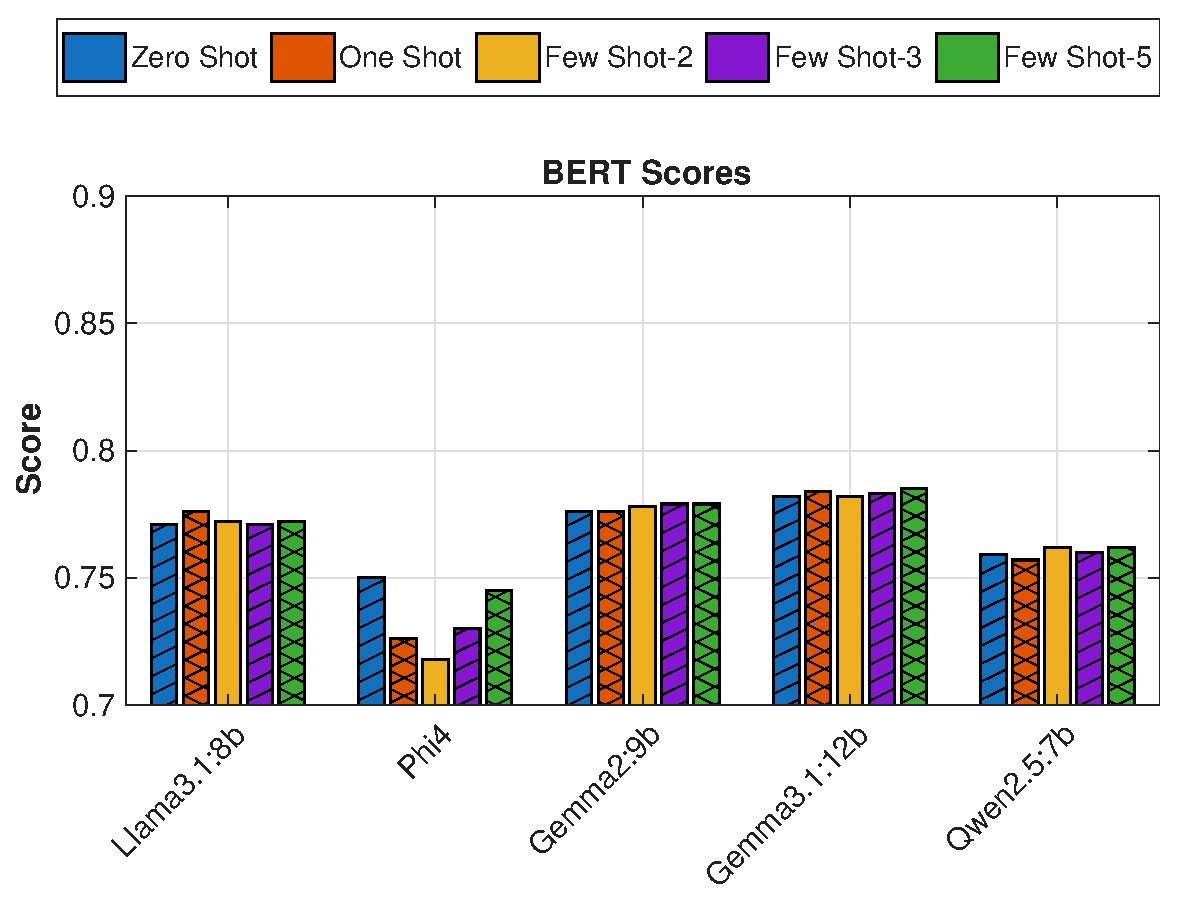
\includegraphics[width=\linewidth]{bert_plot3.eps}
        \caption{BERT Score}
    \end{subfigure}%
    \begin{subfigure}{0.33\textwidth}
        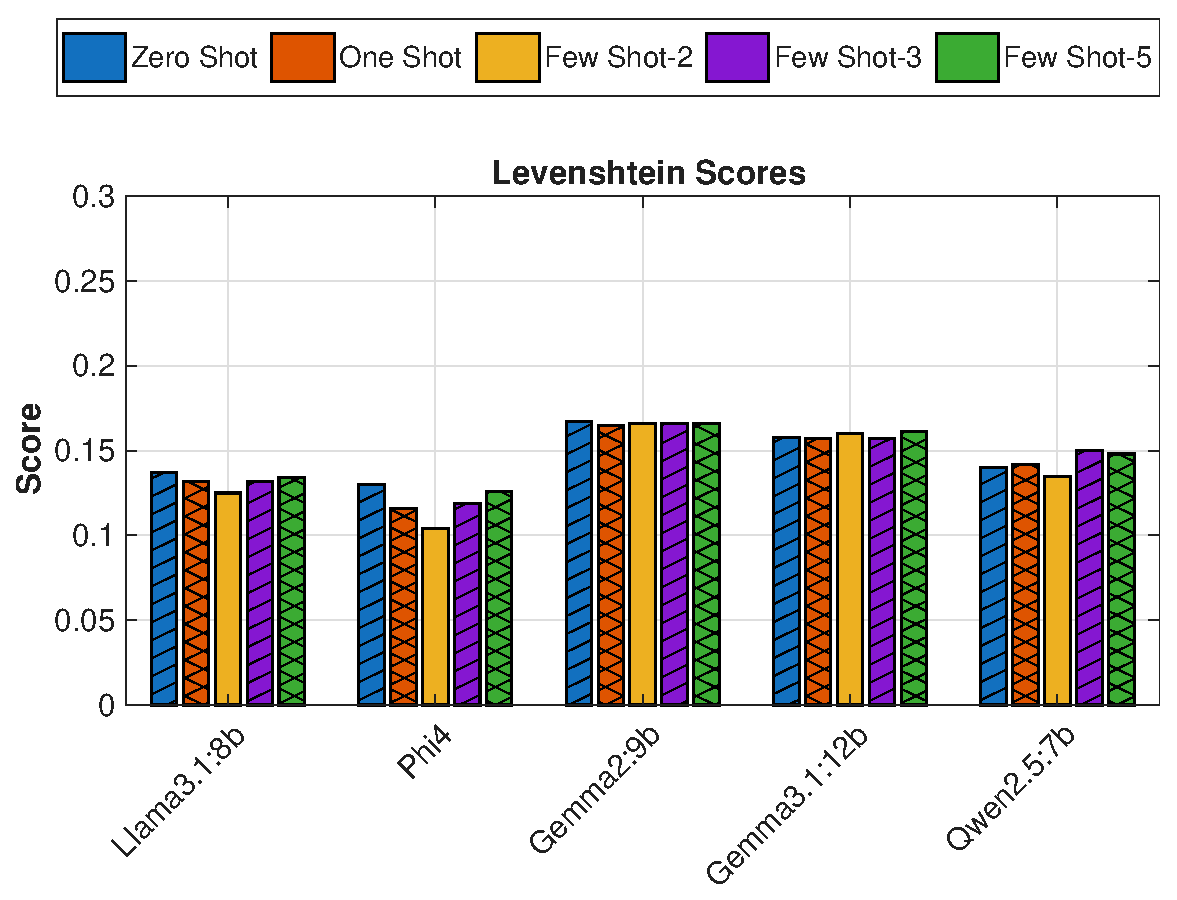
\includegraphics[width=\linewidth]{levenshtein_plot3.eps}
        \caption{Levenshtein Score}
    \end{subfigure}%
    \begin{subfigure}{0.33\textwidth}
        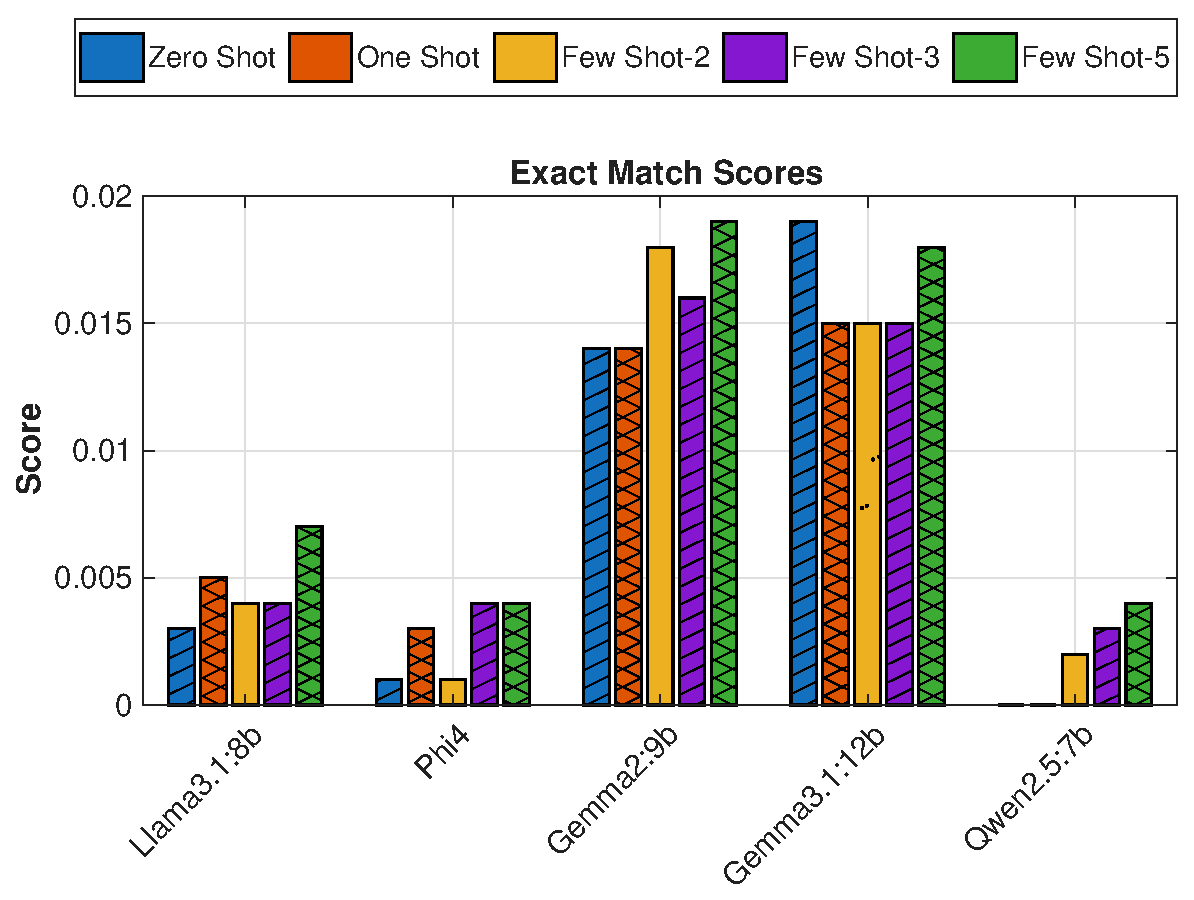
\includegraphics[width=\linewidth]{exact_match_plot3.eps}
        \caption{Exact Match Score}
    \end{subfigure}
    \begin{center}
\begin{center}
\captionof{figure}{\mbox{\small Graphical Representation of the Metric Comparisons for Semantic Similar Selection without CoT}}
\label{fig:semantically-similar-without-cot}
\end{center}

\end{center}

    \vspace{1em}
    
    \begin{subfigure}{0.33\textwidth}
        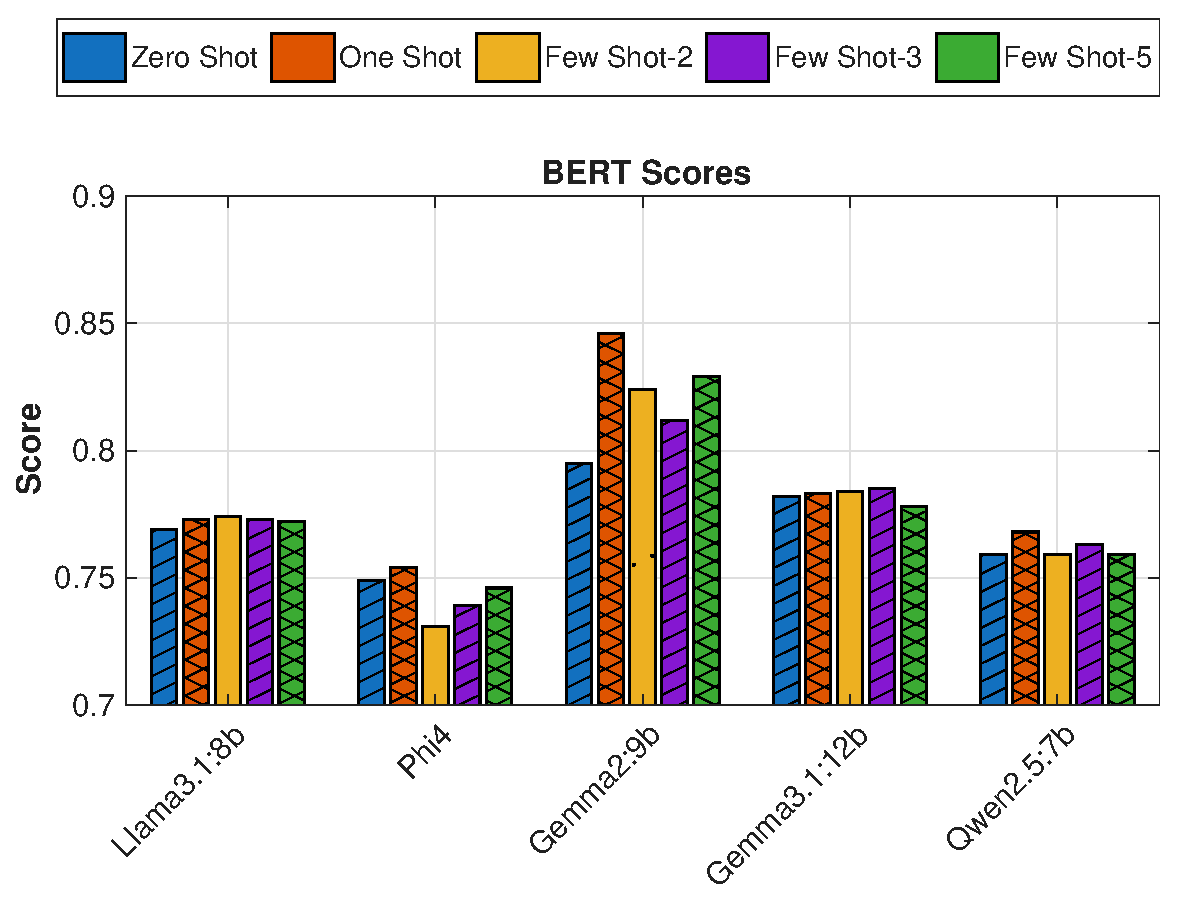
\includegraphics[width=\linewidth]{bert_plot4.eps}
        \caption{BERT Score}
    \end{subfigure}%
    \begin{subfigure}{0.33\textwidth}
        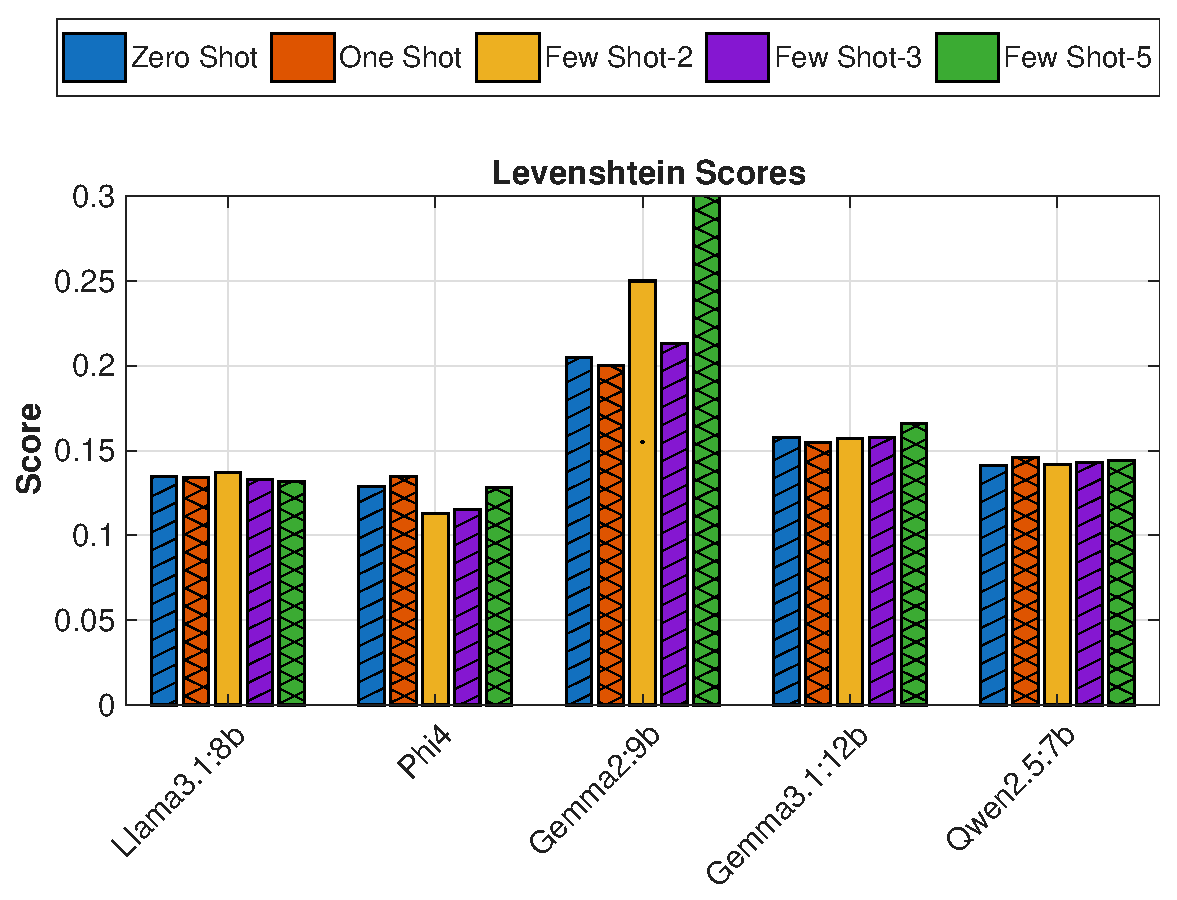
\includegraphics[width=\linewidth]{levenshtein_plot4.eps}
        \caption{Levenshtein Score}
    \end{subfigure}%
    \begin{subfigure}{0.33\textwidth}
        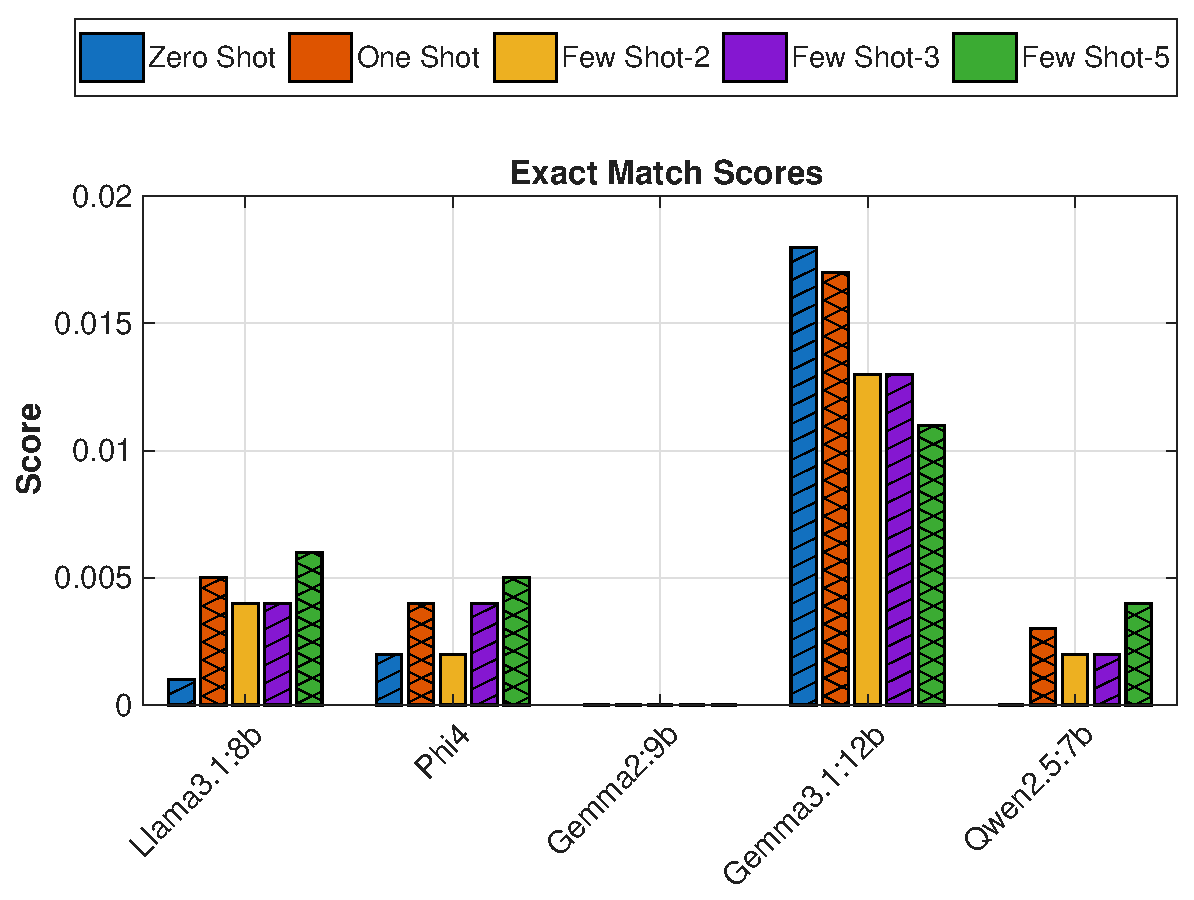
\includegraphics[width=\linewidth]{exact_match_plot4.eps}
        \caption{Exact Match Score}
    \end{subfigure}
    \begin{center}
\captionof{figure}{\mbox{\small Graphical Representation of the Metric Comparisons for Random Selection without CoT}}
\label{fig:random-without-cot}
\end{center}
    \vspace{1em}

    \begin{subfigure}{0.33\textwidth}
        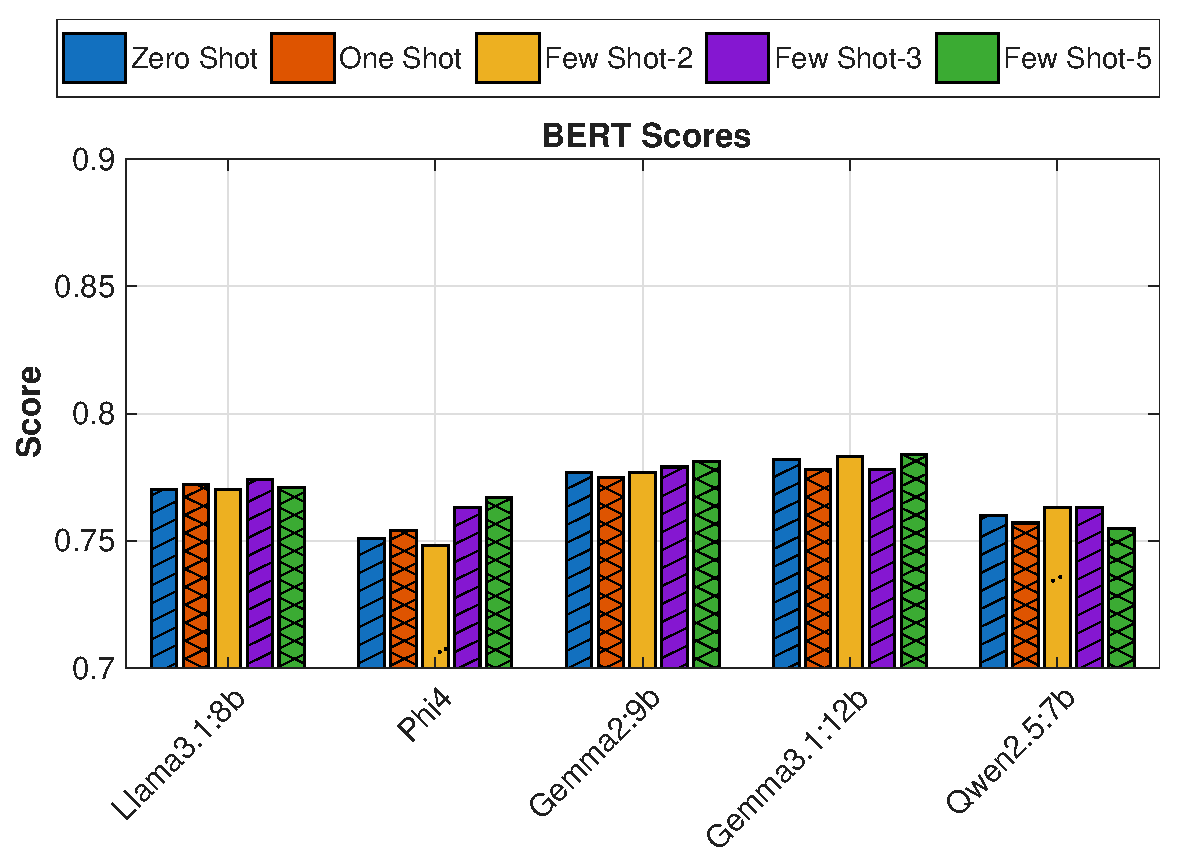
\includegraphics[width=\linewidth]{bert_plot5.eps}
        \caption{BERT Score}
    \end{subfigure}%
    \begin{subfigure}{0.33\textwidth}
        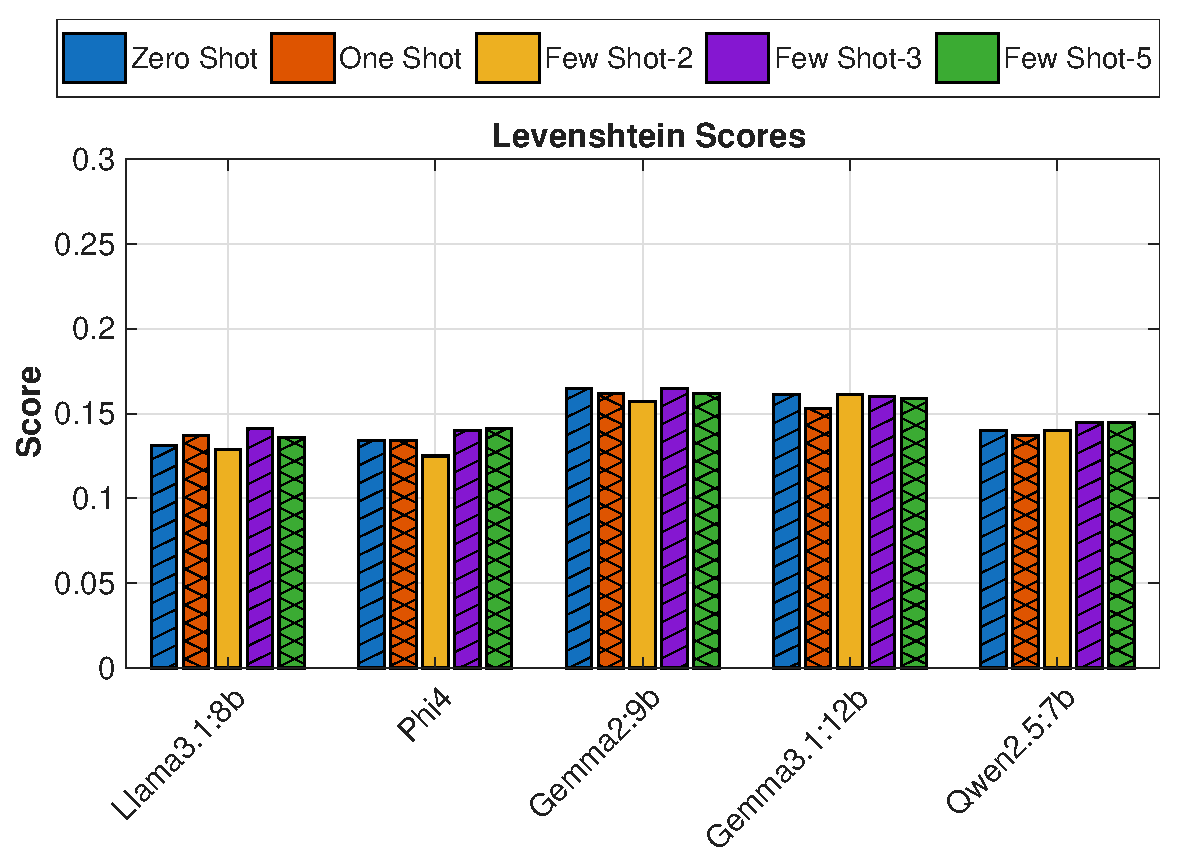
\includegraphics[width=\linewidth]{levenshtein_plot5.eps}
        \caption{Levenshtein Score}
    \end{subfigure}%
    \begin{subfigure}{0.33\textwidth}
        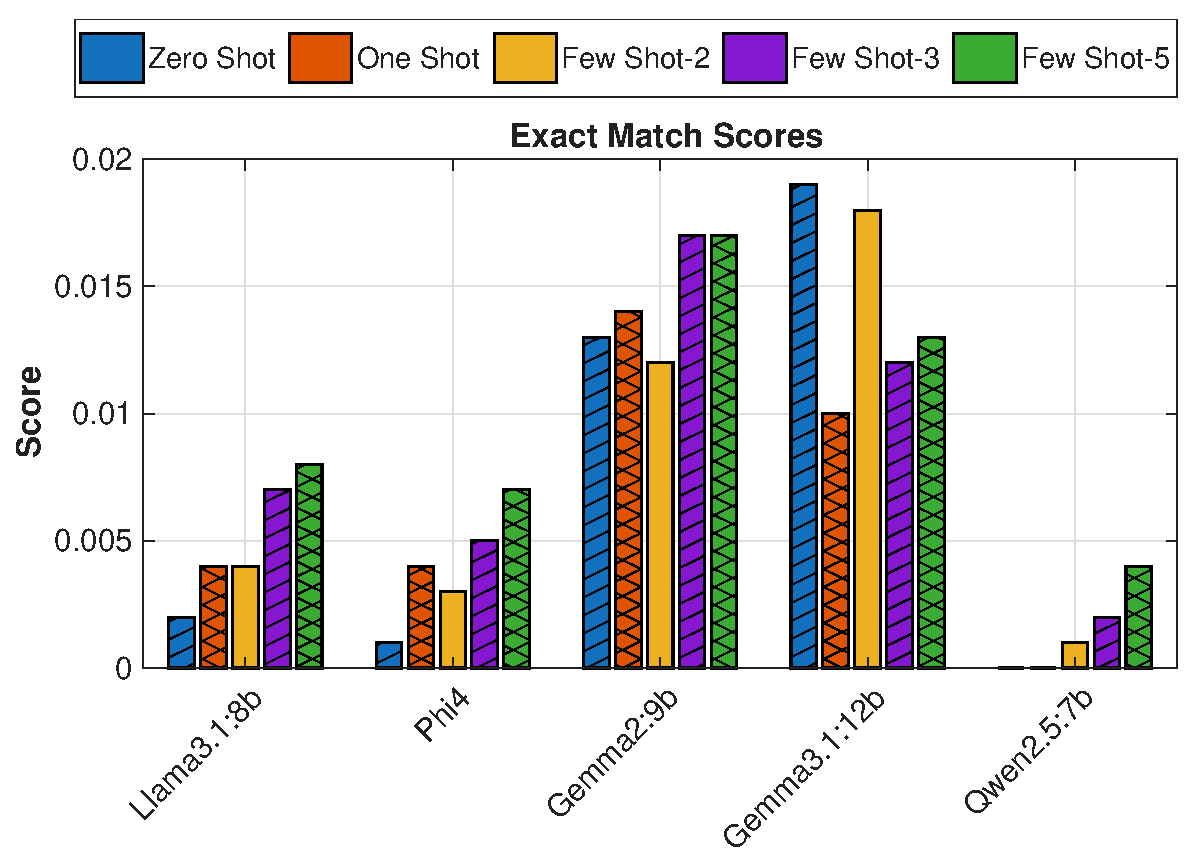
\includegraphics[width=\linewidth]{exact_match_plot5.eps}
        \caption{Exact Match Score}
    \end{subfigure}
   \begin{center}
\captionof{figure}{\mbox{\small Graphical Representation of the Metric Comparisons for Semantic Similar Selection with CoT}}
\label{fig:semantically-similar-with-cot}
\end{center}
    \vspace{1em}

    \begin{subfigure}{0.33\textwidth}
        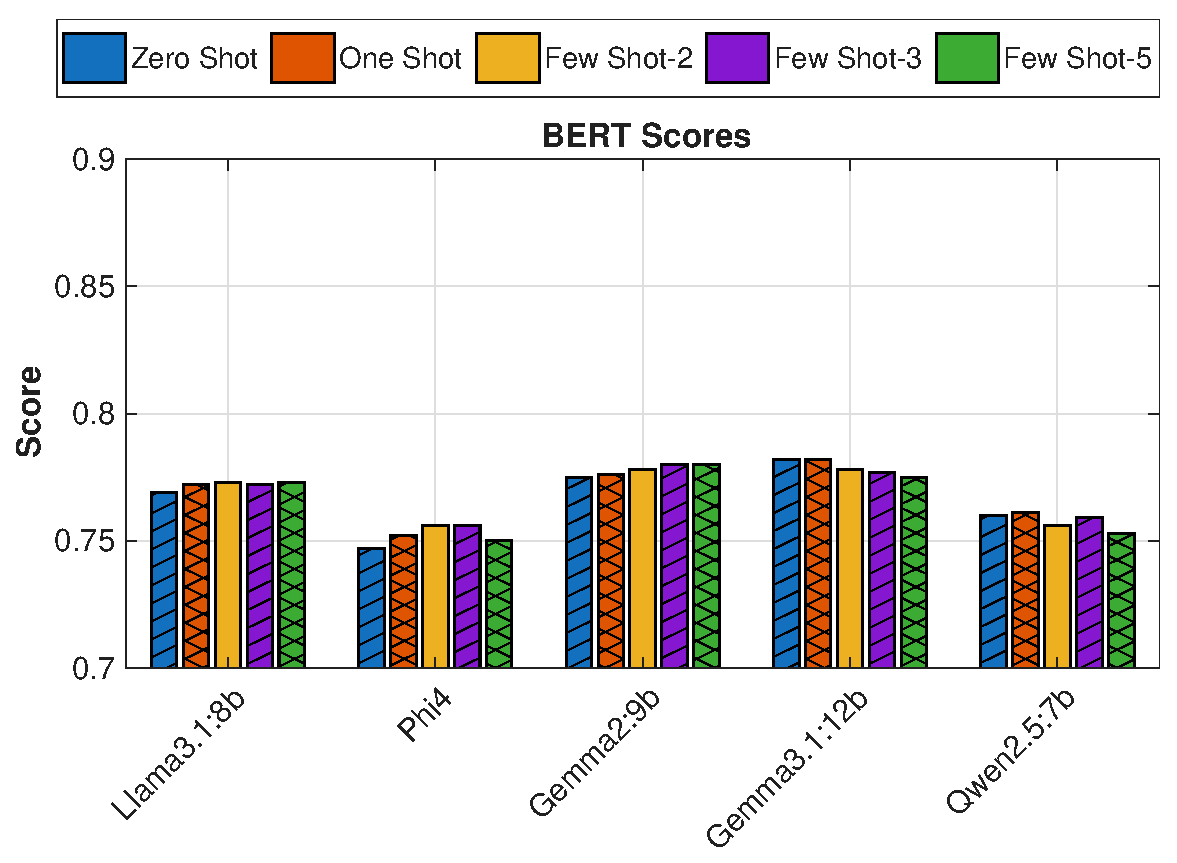
\includegraphics[width=\linewidth]{bert_plot6.eps}
        \caption{BERT Score}
    \end{subfigure}%
    \begin{subfigure}{0.33\textwidth}
        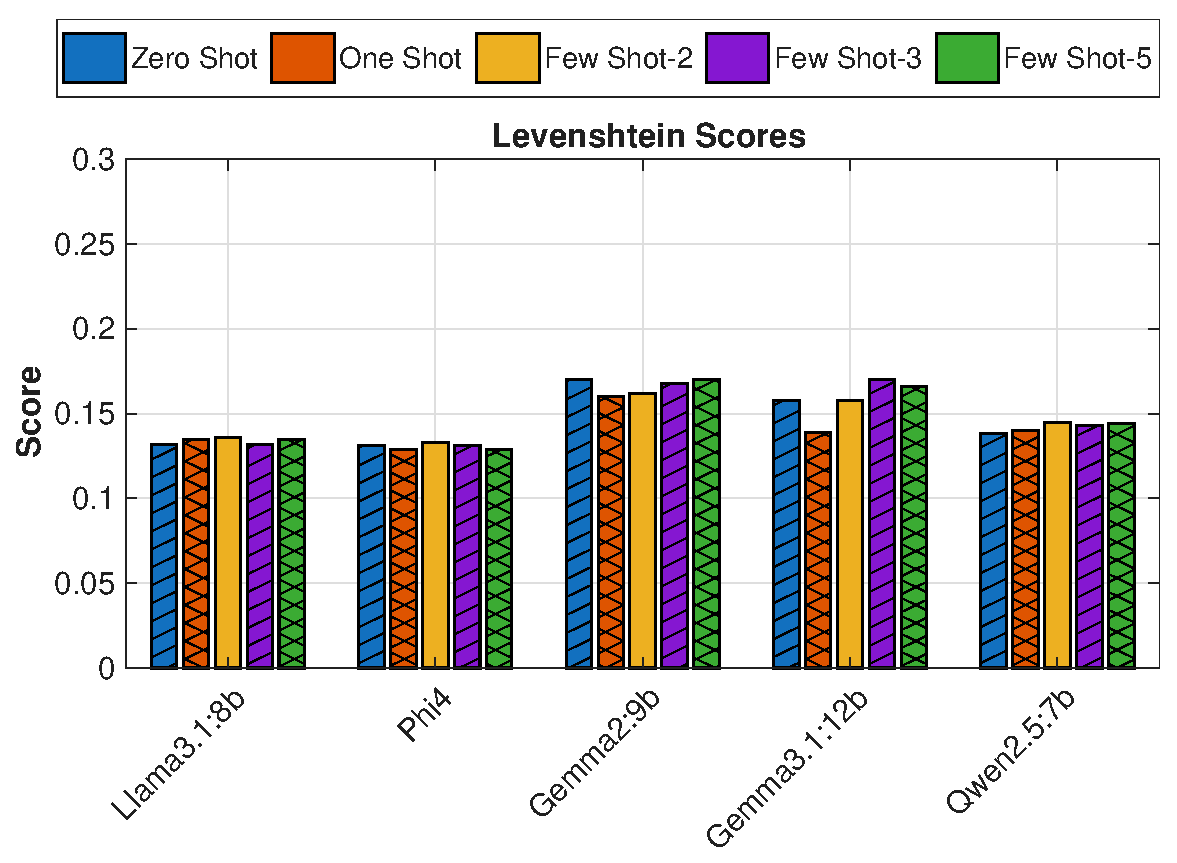
\includegraphics[width=\linewidth]{levenshtein_plot6.eps}
        \caption{Levenshtein Score}
    \end{subfigure}%
    \begin{subfigure}{0.33\textwidth}
        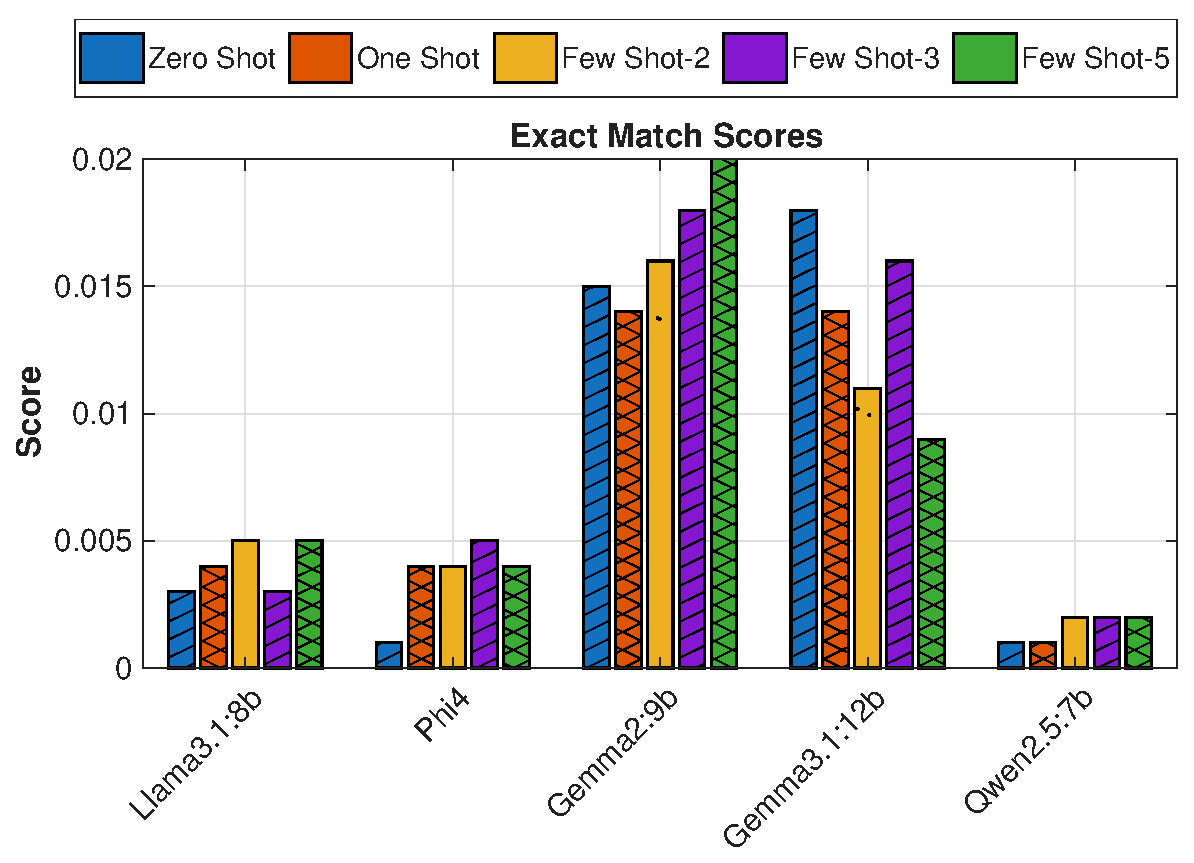
\includegraphics[width=\linewidth]{exact_match_plot6.eps}
        \caption{Exact Match Score}
    \end{subfigure}
    \begin{center}
\captionof{figure}{\mbox{\small Graphical Representation of the Metric Comparisons for Random Selection with CoT}}
\label{fig:random-with-cot}
\end{center}
\end{figure}
\clearpage

\bibliography{papers}
\bibliographystyle{acl_natbib}

\end{document}
